% This is a template for BU-ECE Technical Report.
%
% Depending on report content and author preference, a BU-ECE report may be
% in one of the two following styles:
%
%   - genuine report based on ``report'' style, i.e., with chapters, much like
%     a thesis; can be single- or double-sided,
%
%   - report based on ``article'' style, i.e., with no chapters (only sections,
%     subsections, etc.), much like a journal or conference paper; can be
%     single- or double-sided.

% =====================================================================

%\documentclass[12pt]{report}          %Single-sided report style (chapters)
%\documentclass[12pt,twoside]{report}  %Double-sided report style (chapters)
%\documentclass[12pt]{article}         %Single-sided article style (no chapters)
\documentclass[12pt,twoside]{article} %Double-sided article style (no chapters)

\usepackage{bu_ece_report}

% In case an adjustment of vertical or horizontal margins is needed
% due to particular LaTeX/dvips or OS installation, you can uncomment
% and edit the following definitions.
% -------------------------------------------------------------------
%\topmargin       0.00 in
%\oddsidemargin   0.50 in
%\evensidemargin  0.00 in

\begin{document}

% Definitions.
% ------------
\buecedefinitions%
        {Room Occupancy sensing using a thermal tripwire}
        {Occusense: Intermediate Report}
        {Janis Intoy and Emily Lam}
        {April 10, 2017}
        {2017-01} % Number of the report (four year digits and number) What is the number supposed to be????????

% Box with title to fit the opening in the cover
% (adds an empty page in double-sided printing mode).
% ---------------------------------------------------
\buecereporttitleboxpage

% Title page
% (adds an empty page in double-sided printing mode).
% ---------------------------------------------------
\buecereporttitlepage

% Special page, e.g., if the report is restricted or
% to whom it is dedicated, etc., otherwise skip.
% (adds an empty page in double-sided printing mode).
% ---------------------------------------------------
\bueceprefacepage{Here comes a special preface page. For example, if the report
is restricted, then a suitable note can be included. This page can also be used
to indicate to whom the document is dedicated, etc.}

% Report summary; max. 1 page.
% (adds an empty page in double-sided printing mode).
% ---------------------------------------------------
\pagenumbering{roman}
\setcounter{page}{1}
\buecereportsummary{
The efficiency of HVAC (Heating Ventilation \& Air Conditioning) systems can be improved by making them
adaptive to the number of people in a room. Automatic adjustments to room ventilation and temperature based on 
room occupancy reduces energy use and is more cost efficient.
In order to a estimate a room's occupancy level, the Occusense Senior Design team has created
a reliable, thermal sensor system to capture the motion of people through doorways. We aim to develop
a reliable, real-time algorithm to detect the direction of motion of people passing through in order to track 
the number of people in the room.
}

% Table of contents, list of figures and list of tables.
% ``\bueceemptypage'' adds empty page in double-sided
% printing mode and performs ``\clearpage'' in single-sided
% mode.
% ------------------------------------------------------
\tableofcontents\bueceemptypage
\listoffigures\bueceemptypage
\listoftables\bueceemptypage

% Switch on running headers for the report:
%   odd pages  - title (lowercase); if too long, use
%                the first few words followed by ``...'',
%   even pages - last names of the authors.
% -------------------------------------------------------
\buecereportheaders

% Introduction.
% -------------
\pagenumbering{arabic}
\setcounter{page}{1}

\section{Introduction}  % Article style
%\chapter{Introduction}  % Report style
In modern efficient buildings, controlling the HVAC system preemptively can be a huge cost saver. Therefore, a senior design team at Boston University is working towards developing sensing technology and algorithms to count the number of people in a room so that the system is always conscious of room occupancy and can adjust system parameters, such as ventilation, accordingly before feedback sensing technology can detect abnormalities, such as rising temperatures of a crowded room. There are a number of ways to detect occupancy. However, this project assumes that if a room has a low number of entry points, counting people can be done at the entries based on who is entering or leaving the room. As such, there would be a continuous knowledge of the number of people in a room. The senior design team has implemented a privacy-inclined low resolution thermal sensor with a field of view of 30�x120� positioned at the top of the door frame and looking perpendicularly down. It is capable of capturing a 16x4 pixel array at frame rates of 0.5 to 512 Hz. Using this information, our project is tasked at developing algorithms to count the number of people entering or leaving a room. Specifically, this algorithm will
1) detect the presence of a moving person in the frame and 2) determine the direction of motion.

% Following sections, subsections, etc.
% -------------------------------------
\section{Literature Review}  % Article style
%\chapter{Starting chapter}  % Report style
% Briefly review the literature discussing some other approaches proposed to solve the problem (if any).
Many background subtraction algorithms have been developed to detect changing pixels in a series of images.
A brief review of the more common change detection algorithms can be found in \cite{Goyette14}.
The most successful amongst these incorporate a background model into the algorithm. The use of a model
allows for thresholding of probabilities instead of pixel intensities and is therefore more robust to some variation
in the background scene. In addition, foreground models can improve the sensitivity of the change detectors 
\cite{Elgammal02}. McHugh et al. suggested a foreground model algorithm that is more general as it
is based on spatial neighborhoods. To further improve the discrimination, they also suggest a Markov model
so that labels are more spatially coherent
\cite{Mchugh09}.

\section{Problem Statement}  % Article style
%\section{Early section}  % Report style
% Describe the problem in detail, and the solution proposed, including assumptions, constraints, math formulas, algorithms,
% etc.
Our approach breaks the problem into two parts: 1) detect a person in the doorway and 2) determine the direction of 
motion of the person.

\subsection{Person Detection}
We propose a background subtraction method to detect a person or persons in the frame. In order to accomplish this
we make several assumptions about the acquired data. First, we assume that the background has slow temporal dynamics.
Second, we assume that the data starts with some number of background-only frames. For business and residential 
buildings this is likely true if they close for the night. Finally, we assume that the surface temperature of a single body as 
detected by the sensor has the same variability as the background.
\\ \\
The proposed solution is inspired primarily by the foreground-adaptive background subtraction described in
\cite{Mchugh09}.
The background can be modeled by a probability density function estimated at each pixel location $\mathbf{n}$
from the $N$ most recent pixels that were labeled as background:
$$P_\mathcal{B}\left(I^{(k)} [\mathbf{n}]\right) = \frac{1}{N}\sum_{i \in \mathcal{B}_k[\mathbf{n}]} \mathcal{K}
	\left(I^{(k)}[\mathbf{n}] - I^{(i)}[\mathbf{n}] \right)$$
where 
$I^{(k)}[\mathbf{n}]$ is the temperature at location $\mathbf{n}$,
$B_k[\mathbf{n}]$ are the $N$ previous time indices at which the pixel located at $\mathbf{n}$ was labeled
background, and $\mathcal{K}$ is a zero-mean Gaussian with variance $\sigma^2$. Thresholding these probabilities
with threshold $\theta$ gives an initial classification of pixels into background or foreground.
\\ \\
The development of the foreground model follows a similar formulation, but the summation is over
pixels in the neighborhood of $\mathbf{n}$ that have been already been labeled as foreground. The
likelihood ratio of the probability density functions $P_\mathcal{B}$ and 
$P_\mathcal{F}$ can be thresholded to determine new labels for each pixel. Furthermore,
the number of foreground neighbors a pixel has can be used to adjust the threshold. The more foreground
neighbors a pixel has the easier it is to be labeled as foreground. This will contribute to the spatial
coherency of the labels. Thus, a pixel is labeled as background if
$$\frac{P_\mathcal{B}(I[\mathbf{n}])}{P_\mathcal{F}(I[\mathbf{n}])} > \theta \exp \left(\frac{1}{\gamma} 
	(Q_\mathcal{F}[\mathbf{n}] - Q_\mathcal{B}[\mathbf{n}] )\right)$$
where $Q_\mathcal{F}[\mathbf{n}]$ and $Q_\mathcal{B}[\mathbf{n}]$ are the number of neighbors that are 
foreground and background respectively and $\gamma$ is a parameter to control how strongly the threshold
adapts. The thresholding step can be done iteratively as labels are updated in each step.
\\ \\
This algorithm will result in labels for each pixel in each frame as background or foreground. The number of foreground
pixels in each frame could indicate whether a person is in the frame.

\subsection{Direction Discrimination}
Emily

\section{Implementation}  % Article style
%\chapter{Another chapter}  % Report style
% Describe how you have implemented the proposed solution; include the source code in the appendix.
The current implementation of the algorithm is in Matlab. To integrate with the senior design team it
would need to be ported into Python.

\subsection{Data Acquisition}  % Article style
%\section{New section}  % Report style
The senior design team has a the thermal sensor setup and given us access to record data from it so that we can 
continue to collect data on top of what they have already shared with us. We plan to collect a few trials of realistic
but potentially difficult situations such as a person lingering in the doorway or multiple people passing through
the door in quick succession.
\\ \\
The data is recorded into text files at a rate of 8-12Hz. The data we currently have was recorded at 8Hz
though the Occusense team has updated the sampling rate to 12Hz.

\subsection{Person Detection}
Janis implemented this algorithm in the file backgroundSubtraction.m. It takes as input a structure of parameters
and a 3-D array of temperatures over the two spatial and one time dimensions. This implementation could
be modified to run in real time and, depending on the size of the history for the computation of the background
PDF, would not require too much memory.

\subsection{Direction Discrimination}
Emily

\section{Experimental Results}  % Article style
%\chapter{Final chapter}  % Report style
% Describe the experiments you have conducted and the results you have obtained. Are you results consistent
% with your original goals?
Algorithms are being tested on simulated data generated by randomly concatenating the current data that is labeled.
The temperatures of the frames are shifted for continuity between frames.

\subsection{Background Subtraction}  % Article style
This method seems to work very well in detecting motion even with a background
temperature that is changing slowly over time as shown in Figure ???. Thresholding the number of detected
foreground pixels would be more robust than thresholding the raw temperature values to determine
if a person is in the frame.
\begin{figure}[htb]
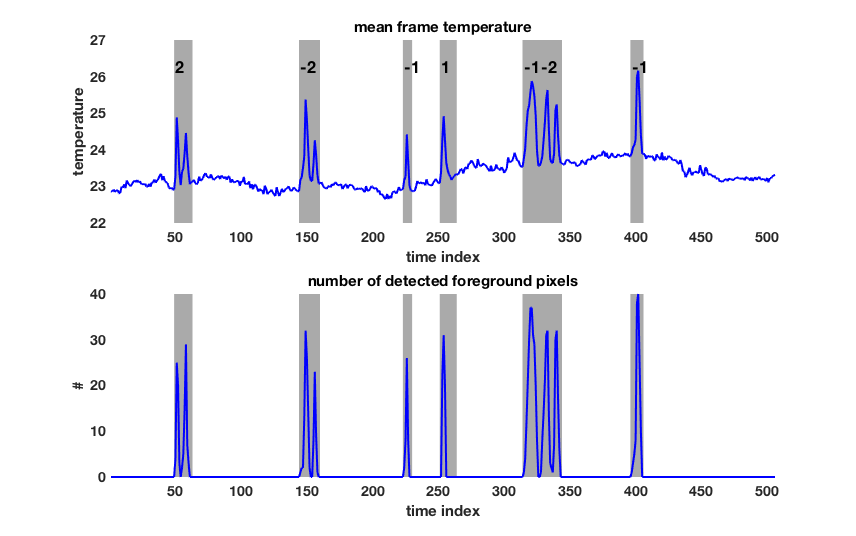
\includegraphics[scale=0.5]{backgroundSubtractionResults.png}
\caption{Comparison of mean frame temperature and number of detected foreground pixels.}
\end{figure}

\section{Conclusions}
% Describe what you have learned from the project and what further improvements are possible.

% Plots (PostScript files) are included through the ``figure'' environment.
% For more complicated figures use the minipage commaned (see LaTeX manual).
% --------------------------------------------------------------------------
%%\begin{figure}[htb]
%%%
%%  \begin{minipage}[t]{0.49\linewidth}\centering
%%%    \centerline{\epsfig{figure=figures/regbsdcod.eps,width=8.0cm}}
%%    \Ovalbox{\vbox to 1.5in{\vfill\hbox{\vtop{\hsize=2.5in\hfill}\hfill}\vfill}}
%%    \medskip
%%    \centerline{(a)}
%%  \end{minipage}\hfill
%%%
%%  \begin{minipage}[t]{0.49\linewidth}\centering
%%%    \centerline{\epsfig{figure=figures/regbsdcod.eps,width=8.0cm}}
%%    \Ovalbox{\vbox to 1.5in{\vfill\hbox{\vtop{\hsize=2.5in\hfill}\hfill}\vfill}}
%%    \medskip
%%    \centerline{(b)}
%%  \end{minipage}
%%
%%  \bigskip
%%
%%  \begin{minipage}[t]{0.49\linewidth}\centering
%%%    \centerline{\epsfig{figure=figures/regbsdcod.eps,width=8.0cm}}
%%    \Ovalbox{\vbox to 1.5in{\vfill\hbox{\vtop{\hsize=2.5in\hfill}\hfill}\vfill}}
%%    \medskip
%%    \centerline{(c)}
%%  \end{minipage}\hfill
%%%
%%  \begin{minipage}[t]{0.49\linewidth}\centering
%%%    \centerline{\epsfig{figure=figures/regbsdcod.eps,width=8.0cm}}
%%    \Ovalbox{\vbox to 1.5in{\vfill\hbox{\vtop{\hsize=2.5in\hfill}\hfill}\vfill}}
%%    \medskip
%%    \centerline{(d)}
%%  \end{minipage}
%%%
%%  \caption{Block diagram: (a) one; (b) two; (c) three, and (d) four.}
%%  \label{fig:example}
%%\end{figure}

% Bibliography.
% -------------
\parskip=0pt
\parsep=0pt
\bibliographystyle{ieeetrsrt}

% Important: substitute your BiBTeX (*.bib) files below.
% ------------------------------------------------------
\bibliography{strings,konrad,manuals}

\end{document}
